\begin{enumerate}[label=\thesection.\arabic*.,ref=\thesection.\theenumi]
\numberwithin{equation}{enumi}

\begin{abstract}
This document contains the solution to a Lines and planes problem.
\end{abstract}
Download all python codes from 
%
\begin{lstlisting}
https://github.com/Jayanth9969/EE5600/blob/master/Assignment1/code.py
\end{lstlisting}

\section{Problem}



Find the Angle between the following lines

\begin{align*}
  \myvec{\sqrt{3}  &  1}\vec{x}=1
\\
    \myvec{1 & \sqrt{3}}\vec{x}=4
\\ \\
\end{align*}

\section{Solution}
The \textbf{Approach} is :
\begin{flushleft}
    For finding the Angle between these lines we will use dot-Product Formula and with  the help of direction vectors we can find angle between these 2 lines.
\end{flushleft}

\begin{enumerate}
    \item We will make direction vectors from these line vectors form:

\begin{align*}
    \vec{m}_1 = \myvec{-\sqrt{3} & 1}\tag{0.1}\\
    \vec{m}_2 = \myvec{-1 & \sqrt{3}}\tag{0.2}\\
\end{align*} 


Now we will find out magnitudes of each vectors $\vec{m}_1$,$\vec{m}_2$ :

\begin{align*}
    \norm{\vec{m}_1} = \sqrt{3+1} = 2\tag{1.1}\\
    \norm{\vec{m}_2} = \sqrt{1+3} = 2\tag{1.2}\\
\end{align*}

Thus angle between 2 vectors $\vec{m}_1$,$\vec{m}_2$ can be found using dot-product using the formula below,\\
Let $\theta$ be angle between vectors $\vec{m}_1$,$\vec{m}_2$ then,\\
\begin{align*}
    \theta = \arccos({\frac{\vec{m}_1^{T}\vec{m}_2}{\norm{\vec{m_1}}.\norm{\vec{m}_2}}})\tag{2}
\end{align*}

By,Putting values into above equation we,get\\\\
\begin{align*}
    \theta &= \arccos(\frac{\myvec{-\sqrt{3}&1}^{T}\myvec{-1&\sqrt{3}}}{\big{2\times2}})\tag{3.1}\\\\
    \theta &= \arccos({\frac{2\times\sqrt{3}}{4}})\tag{3.2}\\\\
    \theta &= \arccos({\frac{\sqrt{3}}{2}})\tag{3.3}\\\\
    \theta &= 30\degree\tag{3.4}\\\\
\end{align*}
Thus the angle between given lines is 30\degree\\\\

\renewcommand{\thefigure}{\theenumi.\arabic{figure}}
\begin{figure}[!ht]
    \centering
    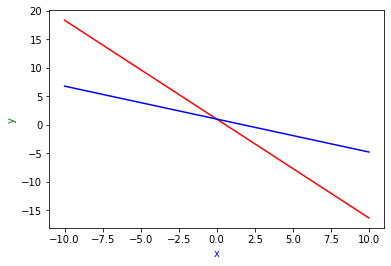
\includegraphics[width=\columnwidth]{Figure_1.png}
    \caption{Figure}
% \label{fig: Fig}
\end{figure}
% \item We converted these line vectors in augmented matrix form: 

% \begin{align*}
%     \myvec{3 & -1 & \vrule & 3\\9 & -3 & \vrule & 9}
% \\
%     \xleftrightarrow[]{R_{2}=\frac{R_{2}}{3}} \myvec{1 & -1 & \vrule & 3\\1 & -1 & \vrule & 3}
% \end{align*}

% As $R_{1}=R_{2}$ , left part can never be converted into a identity matrix , and we can see now both row are same that means both lines are same they intersect at infinitely many points.

% \renewcommand{\thefigure}{\theenumi.\arabic{figure}}
% \begin{figure}[!ht]
%     \centering
%     \includegraphics[width=\columnwidth]{./figures/A1_partc}
% \caption{part(c)}
% \label{fig: part(c)}
% \end{figure}

% \item We converted these line vectors in augmented matrix form: 

% \begin{align*}
%     \myvec{0.2 & 0.3 & \vrule & 1.3\\0.4 & 0.5 & \vrule & 2.3}
% \\
%     \xleftrightarrow[]{R_{2}=R_{2}-2\times R_{1}} \myvec{0.2 & 0.3 & \vrule & 1.3\\0 & -0.1 & \vrule & -0.3}
% \\
%     \xleftrightarrow[]{R_{2}=\frac{R_{2}}{-0.1}} \myvec{0.2 & 0.3 & \vrule & 1.3\\0 & 1 & \vrule & 3}
% \\
%     \xleftrightarrow[]{R_{1}=R_{1}-0.3 \times R_{2}} \myvec{0.2 & 0 & \vrule & 0.4\\0 & 1 & \vrule & 3}
% \\
%     \xleftrightarrow[]{R_{1}=\frac{R_{1}}{0.2}} \myvec{1 & 0 & \vrule & 2\\0 & 1 & \vrule & 3}
% \end{align*}

% As left part is converted into a identity matrix the intersection vector is \myvec{2 \\ 3}

% \renewcommand{\thefigure}{\theenumi.\arabic{figure}}
% \begin{figure}[!ht]
%     \centering
%     \includegraphics[width=\columnwidth]{./figures/A1_partd}
% \caption{part(d)}
% \label{fig: part(d)}
% \end{figure}

% \item We converted these line vectors in augmented matrix form:

% \begin{align*}
%     \myvec{\sqrt{2} & \sqrt{3} & \vrule & 0\\\sqrt{3} & \sqrt{8} & \vrule & 0}
% \\
%     \xleftrightarrow[]{R_{2}=R_{2}-\frac{\sqrt{3}}{\sqrt{2}}\times R_{1}} \myvec{\sqrt{2} & \sqrt{3} & \vrule & 0\\0 & \cfrac{1}{\sqrt{2}} & \vrule & 0}
% \end{align*}

% As we see whatever operation we are applying last column of our augmented matrix remains zero.So the lines are homogeneous lines and they always pass through  origin , the intersection vector is \myvec{0 \\ 0}

% \renewcommand{\thefigure}{\theenumi.\arabic{figure}}
% \begin{figure}[!ht]
%     \centering
%     \includegraphics[width=\columnwidth]{./figures/A1_parte}
% \caption{part(e)}
% \label{fig: part(e)}
% \end{figure}

% \item We converted these line vectors in augmented matrix form: 

% \begin{align*}
%     \myvec{\cfrac{3}{2} & \cfrac{-5}{3} & \vrule & -2\\\cfrac{1}{3} & \cfrac{1}{2} & \vrule & \cfrac{13}{6}}
% \\
%     \xleftrightarrow[]{R_{1}=6\times R_{1}}
%     \xleftrightarrow[]{R_{2}=6\times R_{2}} \myvec{9 & -10 & \vrule & -12\\2 & 3 & \vrule & 13}
% \\
%     \xleftrightarrow[]{R_{1}=R_{1}-4\times R_{2}} \myvec{1 & -22 & \vrule & -64\\2 & 3 & \vrule & 13}
% \\
%     \xleftrightarrow[]{R_{2}=R_{2}-2\times R_{1}}  \myvec{1 & -22 & \vrule & -64\\0 & 47 & \vrule & 141}
% \\
%     \xleftrightarrow[]{R_{2}=\frac{R_{2}}{47}}  \myvec{1 & -22 & \vrule & -64\\0 & 1 & \vrule & 3}
% \\
%     \xleftrightarrow[]{R_{1}=R_{1}+22\times R_{2}} \myvec{1 & 0 & \vrule & 2\\0 & 1 & \vrule & 3}
% \end{align*}

% As left part is converted into a identity matrix the intersection vector is \myvec{2 \\ 3}

% \renewcommand{\thefigure}{\theenumi.\arabic{figure}}
% \begin{figure}[!ht]
%     \centering
%     \includegraphics[width=\columnwidth]{./figures/A1_partf}
% \caption{part(f)}
% \label{fig: part(f)}
% \end{figure}

\end{enumerate}

\end{enumerate}